\chapter{Discretization + Classification}
\label{chap:experiment1}

\section*{Objective}
To build a classification model for predicting the class of a student based on his course marks.

\section*{Procedure}
\begin{itemize}
\item Marks of all languages and subjects have already been discretized as in ~/ref{}
\item Built a classification model using a decision tree algorithm with L1{\_}CLASS, L2{\_}CLASS, L3{\_}CLASS, S1{\_}CLASS, S2{\_}CLASS, S3{\_}CLASS as predictors.
\begin{itemize}
\item Proportion of sizes of the training and test data sets were respectively 2/3 and 1/3.
\item Data records themselves were put into both the above data sets using random sampling.
\end{itemize}
\end{itemize}

\section*{Observations}
\begin{itemize}
\item Tabulation of the count of the predicted versus actual values for the test data set
\begin{lstlisting}
{
      pred
true      1    2 D    FAIL PASS
  1    2717  299   50    1    9
  2     613  920    0   23  350
  D     212    1  274    0    0
  FAIL    9   49    0 1894  558
  PASS   58  458    0  424 2081
}
\end{lstlisting}
\item Misclassification error
\begin{lstlisting}
0.2830909
\end{lstlisting}
\item Decision tree generated
\begin{figure}[h!]
  \caption{Decision Tree}
  \centering
    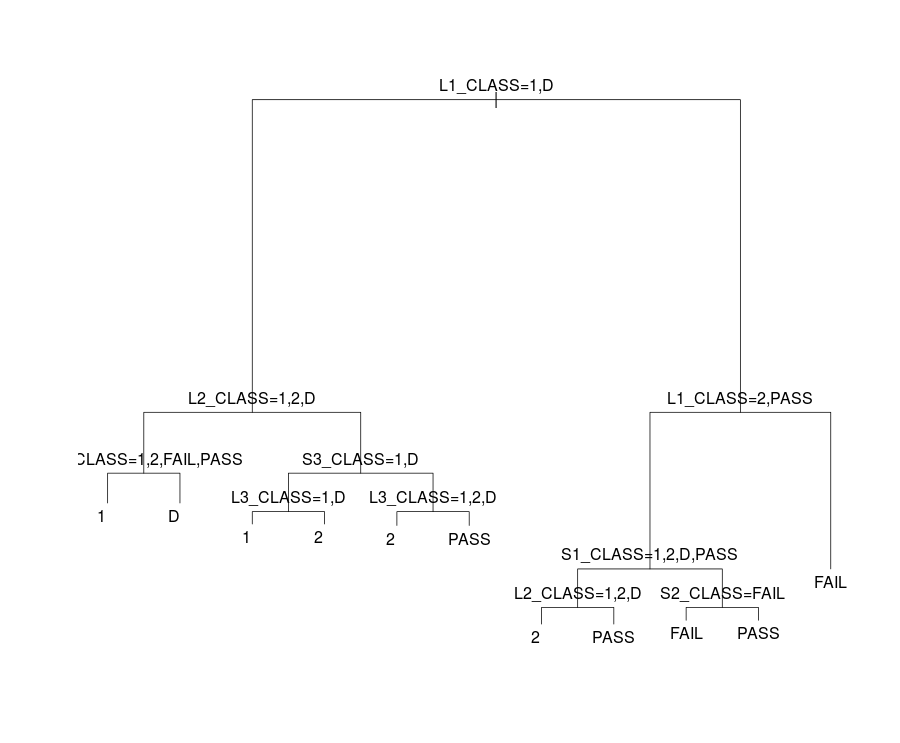
\includegraphics[scale=0.4]{img/rpart_nrc_class.png}
\end{figure}
\end{itemize}

\section*{Conclusions}
TODO